\vfill
\begin{columns}[b]
  \begin{column}{0.45\linewidth}
    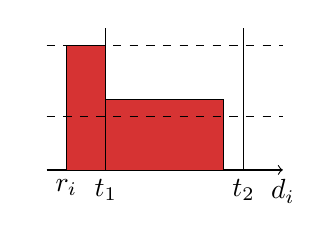
\begin{tikzpicture} [xscale=0.5,yscale=0.45]
      \node (O) at (0,0) {};
      \draw [->] (0,0) -- (6,0);
      \fill[red!80!black!80] (0.5,0) rectangle (1.5,3.5);
      \fill[red!80!black!80] (1.5,0) rectangle (4.5,2);
      \draw (0.5,0) node[below] {$r_i$};
      \draw (6,0) node[below] {$d_i$};
      \draw (1.5,0) node[below] {$t_1$} -- (1.5,4);
      \draw (5,0) node[below] {$t_2$} -- (5,4);
      \draw[dashed] (0,1.5) node[left] {$\bmin$} -- (6,1.5);
      \draw[dashed] (0,3.5) node[left] {$\bmax$} -- (6,3.5);
      \draw (0.5,0) -- (0.5,3.5) -- (1.5,3.5) -- (1.5,2) -- 
      (4.5,2) -- (4.5,0);
    \end{tikzpicture}
    \begin{center}
      {\small left-shifted}
    \end{center}
  \end{column}
\hfill  
\begin{column}{0.45\linewidth}  
  \onslide<2->{
      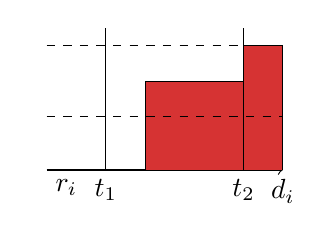
\begin{tikzpicture} [xscale=0.5,yscale=0.45]
        \node (O) at (0,0) {};
        \draw [->] (0,0) -- (6,0);
        \fill[red!80!black!80] (5,0) rectangle (6,3.5);
        \fill[red!80!black!80] (5,0) rectangle (2.5,2.5);
        \draw (0.5,0) node[below] {$r_i$};
        \draw (6,0) node[below] {$d_i$};
        \draw (1.5,0) node[below] {$t_1$} -- (1.5,4);
        \draw (5,0) node[below] {$t_2$} -- (5,4);
        \draw[dashed] (0,1.5) node[left] {$\bmin$} -- (6,1.5);
        \draw[dashed] (0,3.5) node[left] {$\bmax$} -- (6,3.5);
        \draw (6,0) -- (6,3.5) -- (5,3.5) -- (5,2.5) --
        (2.5,2.5) -- (2.5,0);
      \end{tikzpicture}        
      \begin{center}
        {\small right-shifted}
      \end{center}
    }
  \end{column}
\end{columns}
\vfill
\begin{columns}[b]
  \begin{column}{0.45\linewidth}
    \onslide<3->{
      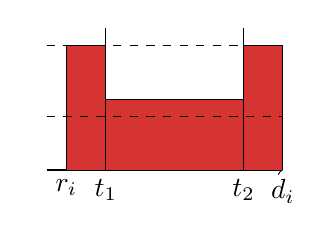
\begin{tikzpicture} [xscale=0.5,yscale=0.45]
        \node (O) at (0,0) {};
        \draw [->] (0,0) -- (6,0);
        \fill[red!80!black!80] (0.5,0) rectangle (1.5,3.5);
        \fill[red!80!black!80] (6,0) rectangle (5,3.5);
        \fill[red!80!black!80] (5,0) rectangle (1.5,2);
        \draw (0.5,0) node[below] {$r_i$};
        \draw (6,0) node[below] {$d_i$};
        \draw (1.5,0) node[below] {$t_1$} -- (1.5,4);
        \draw (5,0) node[below] {$t_2$} -- (5,4);
        \draw[dashed] (0,1.5) node[left] {$\bmin$} -- (6,1.5);
        \draw[dashed] (0,3.5) node[left] {$\bmax$} -- (6,3.5);
        \draw (0.5,0) -- (0.5,3.5) -- (1.5,3.5) -- (1.5,2) --
        (5,2) -- (5,3.5) -- (6,3.5) -- (6,0) ;
      \end{tikzpicture} 
      \begin{center}
      {\small both-shifted 1}
    \end{center}}
  \end{column}
  \hfill
\begin{column}{0.45\linewidth}
    \begin{overlayarea}{0.45\linewidth}{3.5cm}
      \only<4>{
        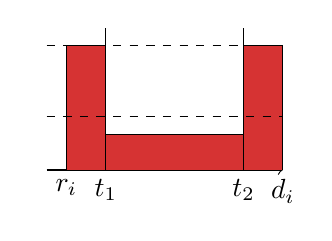
\begin{tikzpicture} [xscale=0.5,yscale=0.45]
          \node (O) at (0,0) {};
          \draw [->] (0,0) -- (6,0);
          \fill[red!80!black!80] (0.5,0) rectangle (1.5,3.5);
          \fill[red!80!black!80] (6,0) rectangle (5,3.5);
          \fill[red!80!black!80] (5,0) rectangle (1.5,1);
          \draw (0.5,0) node[below] {$r_i$};
          \draw (6,0) node[below] {$d_i$};
          \draw (1.5,0) node[below] {$t_1$} -- (1.5,4);
          \draw (5,0) node[below] {$t_2$} -- (5,4);
          \draw[dashed] (0,1.5) node[left] {$\bmin$} -- (6,1.5);
          \draw[dashed] (0,3.5) node[left] {$\bmax$} -- (6,3.5);
          \draw (0.5,0) -- (0.5,3.5) -- (1.5,3.5) -- (1.5,1) --
          (5,1) -- (5,3.5) -- (6,3.5) -- (6,0) ;
        \end{tikzpicture}
      }
      \only<5-> {
        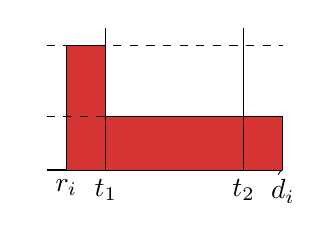
\begin{tikzpicture} [xscale=0.5,yscale=0.45]
          \node (O) at (0,0) {};
          \draw [->] (0,0) -- (6,0);
          \fill[red!80!black!80] (0.5,0) rectangle (1.5,3.5);
          \fill[red!80!black!80] (6,0) rectangle (1.5,1.5);
          \draw (0.5,0) node[below] {$r_i$};
          \draw (6,0) node[below] {$d_i$};
          \draw (1.5,0) node[below] {$t_1$} -- (1.5,4);
          \draw (5,0) node[below] {$t_2$} -- (5,4);
          \draw[dashed] (0,1.5) node[left] {$\bmin$} -- (6,1.5);
          \draw[dashed] (0,3.5) node[left] {$\bmax$} -- (6,3.5);
          \draw (0.5,0) -- (0.5,3.5) -- (1.5,3.5) -- (1.5,1.5) --
          (6,1.5)  -- (6,0) ;
        \end{tikzpicture}
      }
      \onslide<4->{
      \begin{center}
        {\small both-shifted 2}
      \end{center}}
    \end{overlayarea}
  \end{column}
\end{columns}
